\PassOptionsToPackage{unicode=true}{hyperref} % options for packages loaded elsewhere
\PassOptionsToPackage{hyphens}{url}
%
\documentclass[]{article}
\usepackage{lmodern}
\usepackage{amssymb,amsmath}
\usepackage{ifxetex,ifluatex}
\usepackage{fixltx2e} % provides \textsubscript
\ifnum 0\ifxetex 1\fi\ifluatex 1\fi=0 % if pdftex
  \usepackage[T1]{fontenc}
  \usepackage[utf8]{inputenc}
  \usepackage{textcomp} % provides euro and other symbols
\else % if luatex or xelatex
  \usepackage{unicode-math}
  \defaultfontfeatures{Ligatures=TeX,Scale=MatchLowercase}
\fi
% use upquote if available, for straight quotes in verbatim environments
\IfFileExists{upquote.sty}{\usepackage{upquote}}{}
% use microtype if available
\IfFileExists{microtype.sty}{%
\usepackage[]{microtype}
\UseMicrotypeSet[protrusion]{basicmath} % disable protrusion for tt fonts
}{}
\IfFileExists{parskip.sty}{%
\usepackage{parskip}
}{% else
\setlength{\parindent}{0pt}
\setlength{\parskip}{6pt plus 2pt minus 1pt}
}
\usepackage{hyperref}
\hypersetup{
            pdftitle={Final Report},
            pdfauthor={Almas K.},
            pdfborder={0 0 0},
            breaklinks=true}
\urlstyle{same}  % don't use monospace font for urls
\usepackage[margin=1in]{geometry}
\usepackage{color}
\usepackage{fancyvrb}
\newcommand{\VerbBar}{|}
\newcommand{\VERB}{\Verb[commandchars=\\\{\}]}
\DefineVerbatimEnvironment{Highlighting}{Verbatim}{commandchars=\\\{\}}
% Add ',fontsize=\small' for more characters per line
\usepackage{framed}
\definecolor{shadecolor}{RGB}{248,248,248}
\newenvironment{Shaded}{\begin{snugshade}}{\end{snugshade}}
\newcommand{\AlertTok}[1]{\textcolor[rgb]{0.94,0.16,0.16}{#1}}
\newcommand{\AnnotationTok}[1]{\textcolor[rgb]{0.56,0.35,0.01}{\textbf{\textit{#1}}}}
\newcommand{\AttributeTok}[1]{\textcolor[rgb]{0.77,0.63,0.00}{#1}}
\newcommand{\BaseNTok}[1]{\textcolor[rgb]{0.00,0.00,0.81}{#1}}
\newcommand{\BuiltInTok}[1]{#1}
\newcommand{\CharTok}[1]{\textcolor[rgb]{0.31,0.60,0.02}{#1}}
\newcommand{\CommentTok}[1]{\textcolor[rgb]{0.56,0.35,0.01}{\textit{#1}}}
\newcommand{\CommentVarTok}[1]{\textcolor[rgb]{0.56,0.35,0.01}{\textbf{\textit{#1}}}}
\newcommand{\ConstantTok}[1]{\textcolor[rgb]{0.00,0.00,0.00}{#1}}
\newcommand{\ControlFlowTok}[1]{\textcolor[rgb]{0.13,0.29,0.53}{\textbf{#1}}}
\newcommand{\DataTypeTok}[1]{\textcolor[rgb]{0.13,0.29,0.53}{#1}}
\newcommand{\DecValTok}[1]{\textcolor[rgb]{0.00,0.00,0.81}{#1}}
\newcommand{\DocumentationTok}[1]{\textcolor[rgb]{0.56,0.35,0.01}{\textbf{\textit{#1}}}}
\newcommand{\ErrorTok}[1]{\textcolor[rgb]{0.64,0.00,0.00}{\textbf{#1}}}
\newcommand{\ExtensionTok}[1]{#1}
\newcommand{\FloatTok}[1]{\textcolor[rgb]{0.00,0.00,0.81}{#1}}
\newcommand{\FunctionTok}[1]{\textcolor[rgb]{0.00,0.00,0.00}{#1}}
\newcommand{\ImportTok}[1]{#1}
\newcommand{\InformationTok}[1]{\textcolor[rgb]{0.56,0.35,0.01}{\textbf{\textit{#1}}}}
\newcommand{\KeywordTok}[1]{\textcolor[rgb]{0.13,0.29,0.53}{\textbf{#1}}}
\newcommand{\NormalTok}[1]{#1}
\newcommand{\OperatorTok}[1]{\textcolor[rgb]{0.81,0.36,0.00}{\textbf{#1}}}
\newcommand{\OtherTok}[1]{\textcolor[rgb]{0.56,0.35,0.01}{#1}}
\newcommand{\PreprocessorTok}[1]{\textcolor[rgb]{0.56,0.35,0.01}{\textit{#1}}}
\newcommand{\RegionMarkerTok}[1]{#1}
\newcommand{\SpecialCharTok}[1]{\textcolor[rgb]{0.00,0.00,0.00}{#1}}
\newcommand{\SpecialStringTok}[1]{\textcolor[rgb]{0.31,0.60,0.02}{#1}}
\newcommand{\StringTok}[1]{\textcolor[rgb]{0.31,0.60,0.02}{#1}}
\newcommand{\VariableTok}[1]{\textcolor[rgb]{0.00,0.00,0.00}{#1}}
\newcommand{\VerbatimStringTok}[1]{\textcolor[rgb]{0.31,0.60,0.02}{#1}}
\newcommand{\WarningTok}[1]{\textcolor[rgb]{0.56,0.35,0.01}{\textbf{\textit{#1}}}}
\usepackage{longtable,booktabs}
% Fix footnotes in tables (requires footnote package)
\IfFileExists{footnote.sty}{\usepackage{footnote}\makesavenoteenv{longtable}}{}
\usepackage{graphicx,grffile}
\makeatletter
\def\maxwidth{\ifdim\Gin@nat@width>\linewidth\linewidth\else\Gin@nat@width\fi}
\def\maxheight{\ifdim\Gin@nat@height>\textheight\textheight\else\Gin@nat@height\fi}
\makeatother
% Scale images if necessary, so that they will not overflow the page
% margins by default, and it is still possible to overwrite the defaults
% using explicit options in \includegraphics[width, height, ...]{}
\setkeys{Gin}{width=\maxwidth,height=\maxheight,keepaspectratio}
\setlength{\emergencystretch}{3em}  % prevent overfull lines
\providecommand{\tightlist}{%
  \setlength{\itemsep}{0pt}\setlength{\parskip}{0pt}}
\setcounter{secnumdepth}{0}
% Redefines (sub)paragraphs to behave more like sections
\ifx\paragraph\undefined\else
\let\oldparagraph\paragraph
\renewcommand{\paragraph}[1]{\oldparagraph{#1}\mbox{}}
\fi
\ifx\subparagraph\undefined\else
\let\oldsubparagraph\subparagraph
\renewcommand{\subparagraph}[1]{\oldsubparagraph{#1}\mbox{}}
\fi

% set default figure placement to htbp
\makeatletter
\def\fps@figure{htbp}
\makeatother


\title{Final Report}
\author{Almas K.}
\date{2020-03-16}

\begin{document}
\maketitle

\hypertarget{introduction}{%
\subsection{Introduction:}\label{introduction}}

Alcohol use has been linked with cognitive impairement in the short term
in a variety of situations such as in operation of a motor vehicle.
Numerous factors have been found to affect a student's performance in a
class, from sleep to diet.One previous study has shown the negative
affect of alcohol on academic achievement in a student dataset from the
United States
\href{https://www.ncbi.nlm.nih.gov/pmc/articles/PMC3026599/}{1}. Thus,
it would be interesting to see if this affect on performance can be
replicated in other datasets and whether time of alcohol consumption
(weekend or weekday) makes a difference.

\hypertarget{data-description}{%
\subsection{Data Description}\label{data-description}}

The datasets are obtained from UCI and is originally from Fabio Pagnotta
and Hossain Mohammad Amran. It contains survey data from Portugese
highschool students in a Math and Portugese class and contains
information on 33 attributes. Each class is its own .csv file, but I
will be focussing on the attributes from the Portugese class dataset as
it contains more students (649 students). Each student makes up each
row. This was generated from a colon separated file I made from the
original txt metadata file.

Below is the entire variable set:

\begin{Shaded}
\begin{Highlighting}[]
\NormalTok{meta_dat <-}\StringTok{ }\KeywordTok{read.delim}\NormalTok{((}\KeywordTok{here}\NormalTok{(}\StringTok{"data"}\NormalTok{,}\StringTok{"student_metadata.txt"}\NormalTok{)),}\DataTypeTok{sep =} \StringTok{";"}\NormalTok{, }\DataTypeTok{header=}\OtherTok{FALSE}\NormalTok{)}
\KeywordTok{colnames}\NormalTok{(meta_dat) <-}\StringTok{ }\KeywordTok{c}\NormalTok{(}\StringTok{"variable"}\NormalTok{,}\StringTok{"description"}\NormalTok{,}\StringTok{"type"}\NormalTok{)}
\NormalTok{knitr}\OperatorTok{:::}\KeywordTok{kable}\NormalTok{(meta_dat, }\DataTypeTok{format=}\StringTok{"markdown"}\NormalTok{)}
\end{Highlighting}
\end{Shaded}

\begin{longtable}[]{@{}lll@{}}
\toprule
\begin{minipage}[b]{0.05\columnwidth}\raggedright
variable\strut
\end{minipage} & \begin{minipage}[b]{0.28\columnwidth}\raggedright
description\strut
\end{minipage} & \begin{minipage}[b]{0.58\columnwidth}\raggedright
type\strut
\end{minipage}\tabularnewline
\midrule
\endhead
\begin{minipage}[t]{0.05\columnwidth}\raggedright
school\strut
\end{minipage} & \begin{minipage}[t]{0.28\columnwidth}\raggedright
student's school\strut
\end{minipage} & \begin{minipage}[t]{0.58\columnwidth}\raggedright
binary: GP for Gabriel Pereira or MS for Mousinho da Silveira\strut
\end{minipage}\tabularnewline
\begin{minipage}[t]{0.05\columnwidth}\raggedright
sex\strut
\end{minipage} & \begin{minipage}[t]{0.28\columnwidth}\raggedright
student's sex\strut
\end{minipage} & \begin{minipage}[t]{0.58\columnwidth}\raggedright
binary: F for female or M for male\strut
\end{minipage}\tabularnewline
\begin{minipage}[t]{0.05\columnwidth}\raggedright
age\strut
\end{minipage} & \begin{minipage}[t]{0.28\columnwidth}\raggedright
student's age\strut
\end{minipage} & \begin{minipage}[t]{0.58\columnwidth}\raggedright
numeric: from 15 to 22\strut
\end{minipage}\tabularnewline
\begin{minipage}[t]{0.05\columnwidth}\raggedright
address\strut
\end{minipage} & \begin{minipage}[t]{0.28\columnwidth}\raggedright
student's home address type\strut
\end{minipage} & \begin{minipage}[t]{0.58\columnwidth}\raggedright
binary: U for urban or R for rural\strut
\end{minipage}\tabularnewline
\begin{minipage}[t]{0.05\columnwidth}\raggedright
famsize\strut
\end{minipage} & \begin{minipage}[t]{0.28\columnwidth}\raggedright
family size\strut
\end{minipage} & \begin{minipage}[t]{0.58\columnwidth}\raggedright
binary: LE3 for less or equal to 3 or GT3 for greater than 3\strut
\end{minipage}\tabularnewline
\begin{minipage}[t]{0.05\columnwidth}\raggedright
Pstatus\strut
\end{minipage} & \begin{minipage}[t]{0.28\columnwidth}\raggedright
parent's cohabitation status\strut
\end{minipage} & \begin{minipage}[t]{0.58\columnwidth}\raggedright
binary: T for living together or A for apart\strut
\end{minipage}\tabularnewline
\begin{minipage}[t]{0.05\columnwidth}\raggedright
Medu\strut
\end{minipage} & \begin{minipage}[t]{0.28\columnwidth}\raggedright
mother's education\strut
\end{minipage} & \begin{minipage}[t]{0.58\columnwidth}\raggedright
numeric: 0 for none, 1 for primary education (4th grade), 2 for 5th to
9th grade, 3 for secondary education or 4 for higher education\strut
\end{minipage}\tabularnewline
\begin{minipage}[t]{0.05\columnwidth}\raggedright
Fedu\strut
\end{minipage} & \begin{minipage}[t]{0.28\columnwidth}\raggedright
father's education\strut
\end{minipage} & \begin{minipage}[t]{0.58\columnwidth}\raggedright
numeric: 0 for none, 1 for primary education (4th grade), 2 for 5th to
9th grade, 3 for secondary education or 4 for higher education\strut
\end{minipage}\tabularnewline
\begin{minipage}[t]{0.05\columnwidth}\raggedright
Mjob\strut
\end{minipage} & \begin{minipage}[t]{0.28\columnwidth}\raggedright
mother's job\strut
\end{minipage} & \begin{minipage}[t]{0.58\columnwidth}\raggedright
nominal: teacher, health care related, civil services
(e.g.~administrative or police), at\_home or other\strut
\end{minipage}\tabularnewline
\begin{minipage}[t]{0.05\columnwidth}\raggedright
Fjob\strut
\end{minipage} & \begin{minipage}[t]{0.28\columnwidth}\raggedright
father's job\strut
\end{minipage} & \begin{minipage}[t]{0.58\columnwidth}\raggedright
nominal: teacher, health care related, civil services
(e.g.~administrative or police), at\_home or other\strut
\end{minipage}\tabularnewline
\begin{minipage}[t]{0.05\columnwidth}\raggedright
reason\strut
\end{minipage} & \begin{minipage}[t]{0.28\columnwidth}\raggedright
reason to choose this school\strut
\end{minipage} & \begin{minipage}[t]{0.58\columnwidth}\raggedright
nominal: close to home, school reputation, course preference or
other\strut
\end{minipage}\tabularnewline
\begin{minipage}[t]{0.05\columnwidth}\raggedright
guardian\strut
\end{minipage} & \begin{minipage}[t]{0.28\columnwidth}\raggedright
student's guardian\strut
\end{minipage} & \begin{minipage}[t]{0.58\columnwidth}\raggedright
nominal: mother, father or other\strut
\end{minipage}\tabularnewline
\begin{minipage}[t]{0.05\columnwidth}\raggedright
traveltime\strut
\end{minipage} & \begin{minipage}[t]{0.28\columnwidth}\raggedright
home to school travel time\strut
\end{minipage} & \begin{minipage}[t]{0.58\columnwidth}\raggedright
numeric: 1 for \textless{}15 min., 2 for 15 to 30 min., 3 for 30 min. to
1 hour, or 4 for \textgreater{}1 hour\strut
\end{minipage}\tabularnewline
\begin{minipage}[t]{0.05\columnwidth}\raggedright
studytime\strut
\end{minipage} & \begin{minipage}[t]{0.28\columnwidth}\raggedright
weekly study time\strut
\end{minipage} & \begin{minipage}[t]{0.58\columnwidth}\raggedright
numeric: 1 for \textless{}2 hours, 2 for 2 to 5 hours, 3 for 5 to 10
hours, or 4 for \textgreater{}10 hours\strut
\end{minipage}\tabularnewline
\begin{minipage}[t]{0.05\columnwidth}\raggedright
failures\strut
\end{minipage} & \begin{minipage}[t]{0.28\columnwidth}\raggedright
number of past class failures\strut
\end{minipage} & \begin{minipage}[t]{0.58\columnwidth}\raggedright
numeric: n if 1\textless{}=n\textless{}3, else 4\strut
\end{minipage}\tabularnewline
\begin{minipage}[t]{0.05\columnwidth}\raggedright
schoolsup\strut
\end{minipage} & \begin{minipage}[t]{0.28\columnwidth}\raggedright
extra educational support\strut
\end{minipage} & \begin{minipage}[t]{0.58\columnwidth}\raggedright
binary: yes or no\strut
\end{minipage}\tabularnewline
\begin{minipage}[t]{0.05\columnwidth}\raggedright
famsup\strut
\end{minipage} & \begin{minipage}[t]{0.28\columnwidth}\raggedright
family educational support\strut
\end{minipage} & \begin{minipage}[t]{0.58\columnwidth}\raggedright
binary: yes or no\strut
\end{minipage}\tabularnewline
\begin{minipage}[t]{0.05\columnwidth}\raggedright
paid\strut
\end{minipage} & \begin{minipage}[t]{0.28\columnwidth}\raggedright
extra paid classes within the course subject (Math or Portuguese)\strut
\end{minipage} & \begin{minipage}[t]{0.58\columnwidth}\raggedright
binary: yes or no\strut
\end{minipage}\tabularnewline
\begin{minipage}[t]{0.05\columnwidth}\raggedright
activities\strut
\end{minipage} & \begin{minipage}[t]{0.28\columnwidth}\raggedright
extra-curricular activities\strut
\end{minipage} & \begin{minipage}[t]{0.58\columnwidth}\raggedright
binary: yes or no\strut
\end{minipage}\tabularnewline
\begin{minipage}[t]{0.05\columnwidth}\raggedright
nursery\strut
\end{minipage} & \begin{minipage}[t]{0.28\columnwidth}\raggedright
attended nursery school\strut
\end{minipage} & \begin{minipage}[t]{0.58\columnwidth}\raggedright
binary: yes or no\strut
\end{minipage}\tabularnewline
\begin{minipage}[t]{0.05\columnwidth}\raggedright
higher\strut
\end{minipage} & \begin{minipage}[t]{0.28\columnwidth}\raggedright
wants to take higher education\strut
\end{minipage} & \begin{minipage}[t]{0.58\columnwidth}\raggedright
binary: yes or no\strut
\end{minipage}\tabularnewline
\begin{minipage}[t]{0.05\columnwidth}\raggedright
internet\strut
\end{minipage} & \begin{minipage}[t]{0.28\columnwidth}\raggedright
Internet access at home\strut
\end{minipage} & \begin{minipage}[t]{0.58\columnwidth}\raggedright
binary: yes or no\strut
\end{minipage}\tabularnewline
\begin{minipage}[t]{0.05\columnwidth}\raggedright
romantic\strut
\end{minipage} & \begin{minipage}[t]{0.28\columnwidth}\raggedright
with a romantic relationship\strut
\end{minipage} & \begin{minipage}[t]{0.58\columnwidth}\raggedright
binary: yes or no\strut
\end{minipage}\tabularnewline
\begin{minipage}[t]{0.05\columnwidth}\raggedright
famrel\strut
\end{minipage} & \begin{minipage}[t]{0.28\columnwidth}\raggedright
quality of family relationships\strut
\end{minipage} & \begin{minipage}[t]{0.58\columnwidth}\raggedright
numeric: from 1 for very bad to 5 for excellent\strut
\end{minipage}\tabularnewline
\begin{minipage}[t]{0.05\columnwidth}\raggedright
freetime\strut
\end{minipage} & \begin{minipage}[t]{0.28\columnwidth}\raggedright
free time after school\strut
\end{minipage} & \begin{minipage}[t]{0.58\columnwidth}\raggedright
numeric: from 1 for very low to 5 for very high\strut
\end{minipage}\tabularnewline
\begin{minipage}[t]{0.05\columnwidth}\raggedright
goout\strut
\end{minipage} & \begin{minipage}[t]{0.28\columnwidth}\raggedright
going out with friends\strut
\end{minipage} & \begin{minipage}[t]{0.58\columnwidth}\raggedright
numeric: from 1 for very low to 5 for very high\strut
\end{minipage}\tabularnewline
\begin{minipage}[t]{0.05\columnwidth}\raggedright
Dalc\strut
\end{minipage} & \begin{minipage}[t]{0.28\columnwidth}\raggedright
workday alcohol consumption\strut
\end{minipage} & \begin{minipage}[t]{0.58\columnwidth}\raggedright
numeric: from 1 for very low to 5 for very high\strut
\end{minipage}\tabularnewline
\begin{minipage}[t]{0.05\columnwidth}\raggedright
Walc\strut
\end{minipage} & \begin{minipage}[t]{0.28\columnwidth}\raggedright
weekend alcohol consumption\strut
\end{minipage} & \begin{minipage}[t]{0.58\columnwidth}\raggedright
numeric: from 1 for very low to 5 for very high\strut
\end{minipage}\tabularnewline
\begin{minipage}[t]{0.05\columnwidth}\raggedright
health\strut
\end{minipage} & \begin{minipage}[t]{0.28\columnwidth}\raggedright
current health status\strut
\end{minipage} & \begin{minipage}[t]{0.58\columnwidth}\raggedright
numeric: from 1 for very bad to 5 for very good\strut
\end{minipage}\tabularnewline
\begin{minipage}[t]{0.05\columnwidth}\raggedright
absences\strut
\end{minipage} & \begin{minipage}[t]{0.28\columnwidth}\raggedright
number of school absences\strut
\end{minipage} & \begin{minipage}[t]{0.58\columnwidth}\raggedright
numeric: from 0 to 93\strut
\end{minipage}\tabularnewline
\begin{minipage}[t]{0.05\columnwidth}\raggedright
G1\strut
\end{minipage} & \begin{minipage}[t]{0.28\columnwidth}\raggedright
first period grade\strut
\end{minipage} & \begin{minipage}[t]{0.58\columnwidth}\raggedright
numeric: from 0 to 20\strut
\end{minipage}\tabularnewline
\begin{minipage}[t]{0.05\columnwidth}\raggedright
G2\strut
\end{minipage} & \begin{minipage}[t]{0.28\columnwidth}\raggedright
second period grade\strut
\end{minipage} & \begin{minipage}[t]{0.58\columnwidth}\raggedright
numeric: from 0 to 20\strut
\end{minipage}\tabularnewline
\begin{minipage}[t]{0.05\columnwidth}\raggedright
G3\strut
\end{minipage} & \begin{minipage}[t]{0.28\columnwidth}\raggedright
final grade\strut
\end{minipage} & \begin{minipage}[t]{0.58\columnwidth}\raggedright
numeric: from 0 to 20, output target\strut
\end{minipage}\tabularnewline
\bottomrule
\end{longtable}

\hypertarget{data-exploration}{%
\subsection{Data Exploration:}\label{data-exploration}}

\hypertarget{correllogram}{%
\subsubsection{Correllogram}\label{correllogram}}

\includegraphics{/Users/almas/Documents/GitHub/Stat547_class/Project/team11_akhan/images/Correllogram.png}
\includegraphics[width=0.8\textwidth,height=\textheight]{images/Correllogram.png}

In this correllogram, we see a variety of factors having an association
with final grades . The colour scheme shows all positive correlations as
blue, and all negative correlations as red.Term 1 grades(t1\_grades) and
term 2 grades(t2\_grades) having the highest correlation with
final\_grades makes sense here, as earlier term grades are correlated
with later term grades. We will mainly focus on the alcohol (workday and
weekend), which show negative correlation.

\hypertarget{boxplots}{%
\subsubsection{Boxplots}\label{boxplots}}

Let's look at weekend alcohol and workday alcohol use's spread.

\includegraphics{/Users/almas/Documents/GitHub/Stat547_class/Project/team11_akhan/images/Final Grade vs Weekend Alcohol.png}
\includegraphics[width=0.8\textwidth,height=\textheight]{images/Final Grade vs Weekend Alcohol.png}~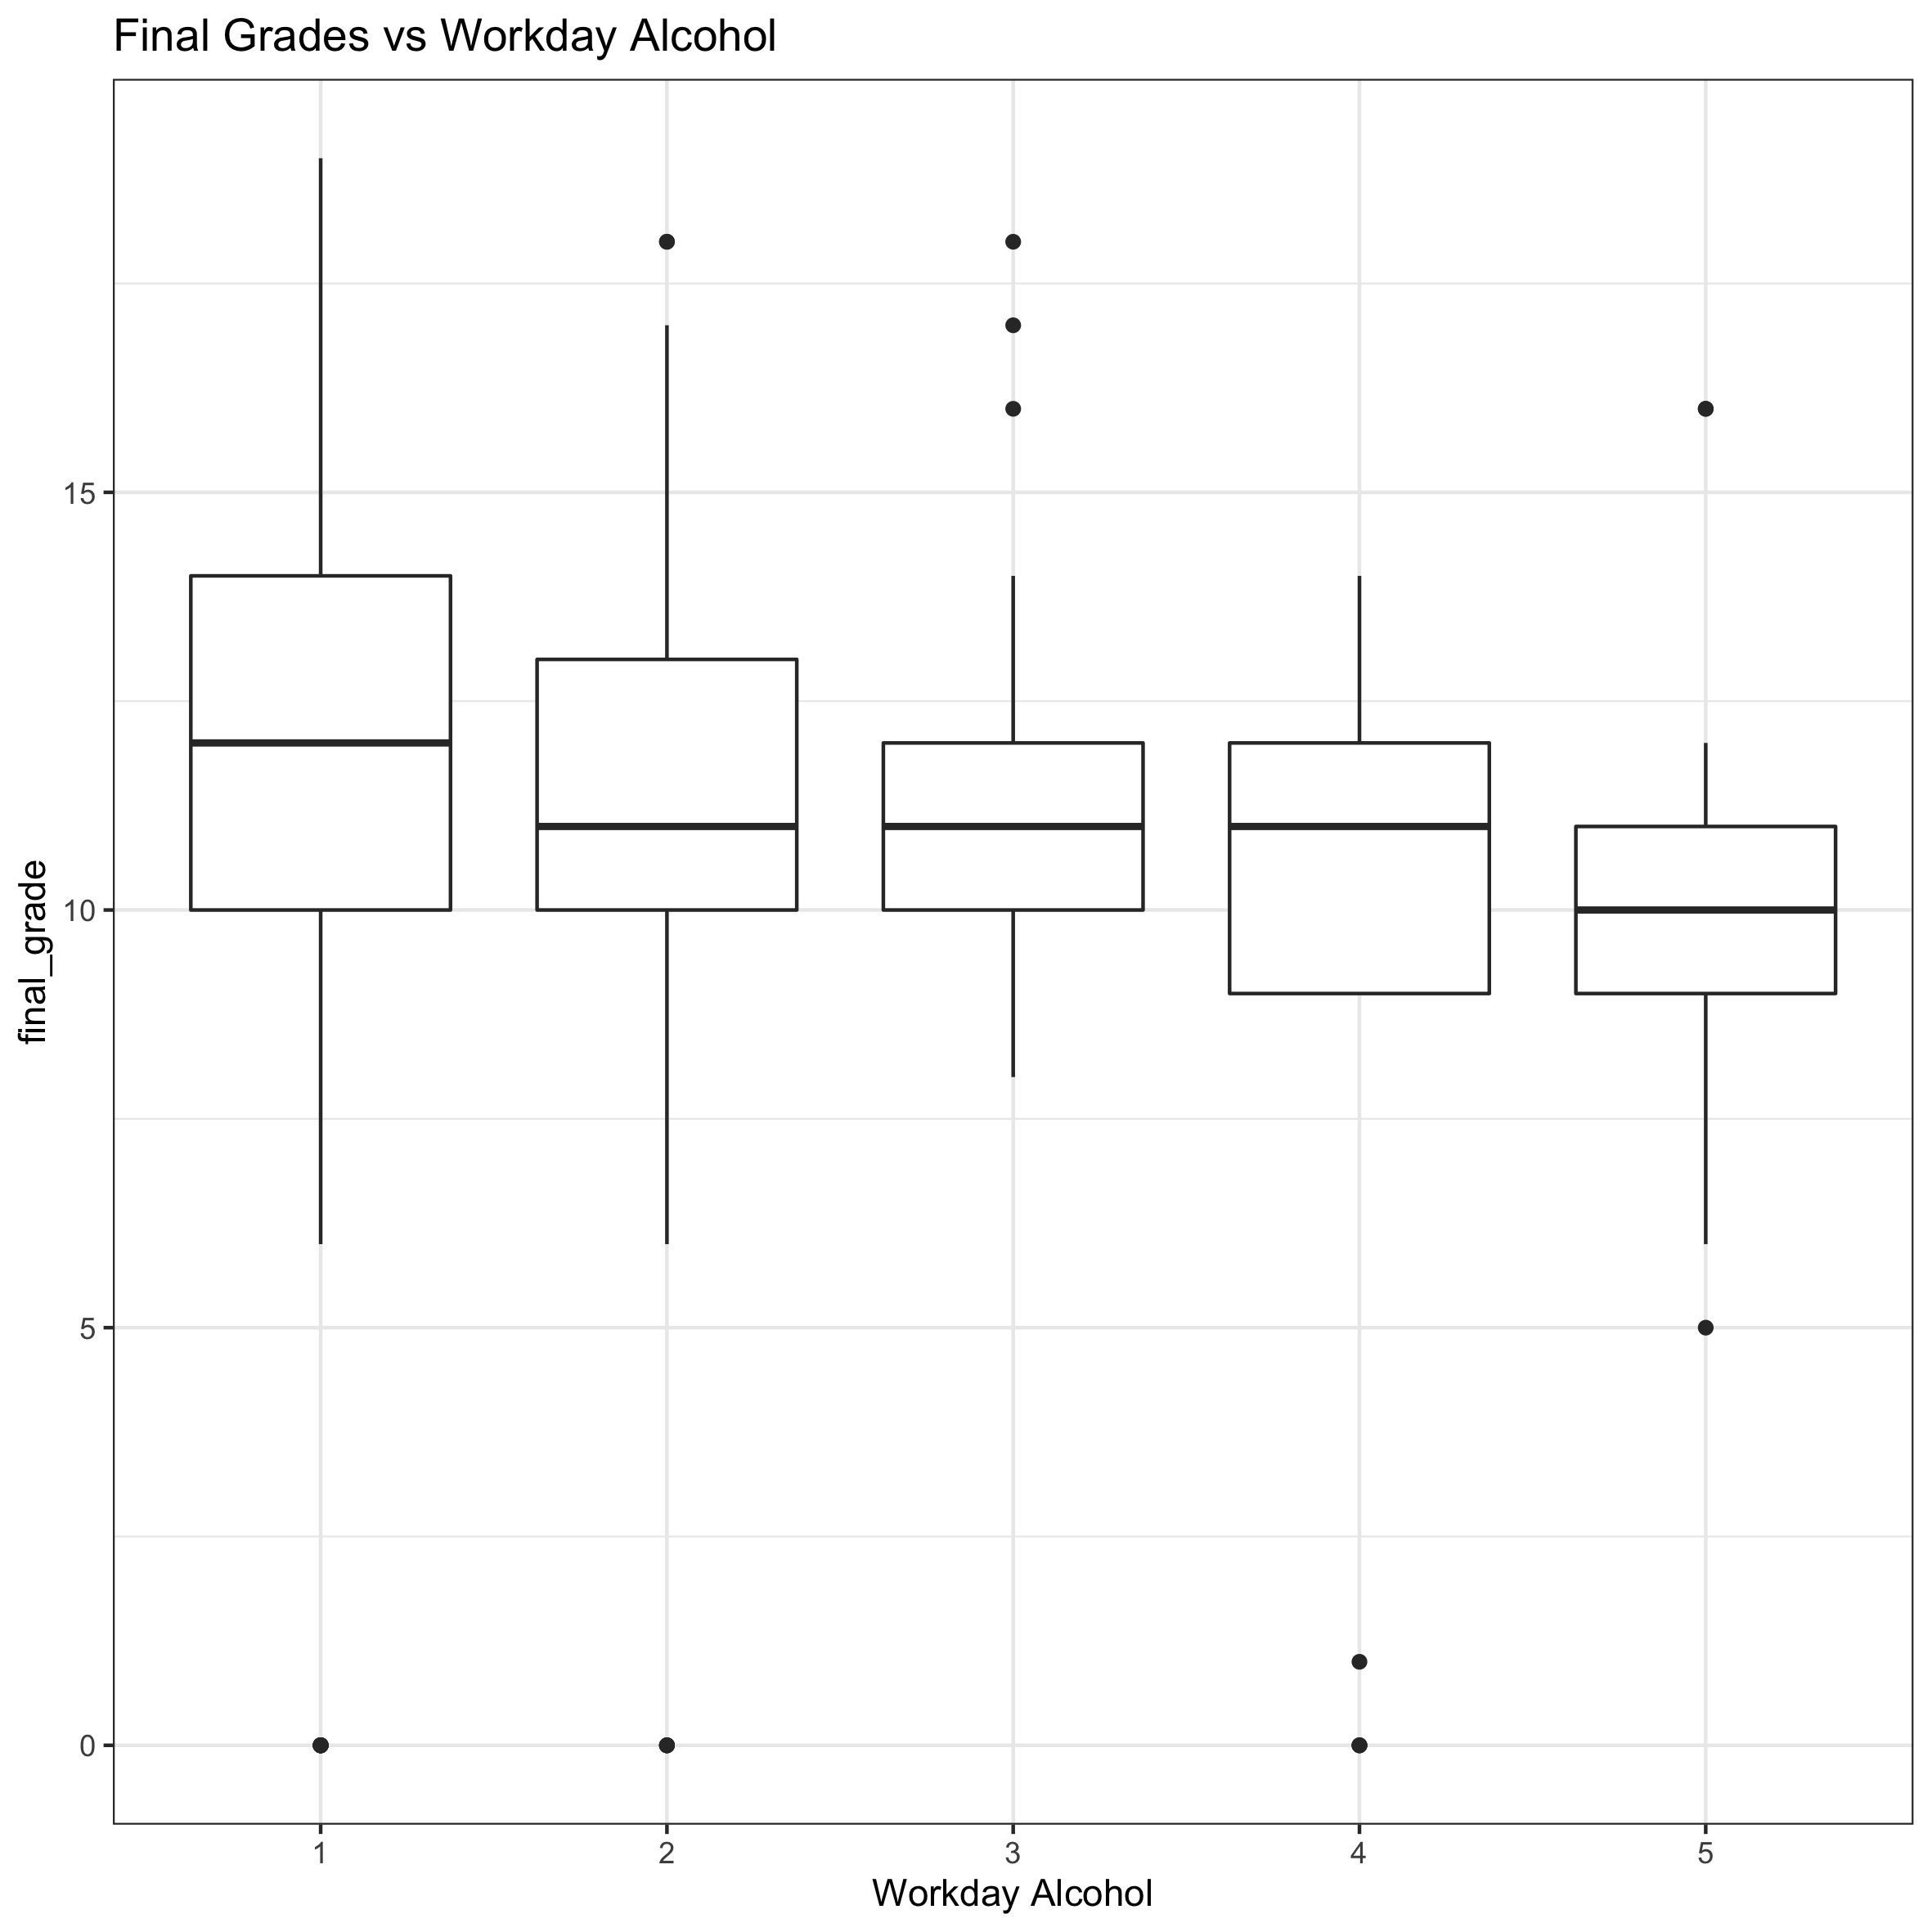
\includegraphics[width=0.8\textwidth,height=\textheight]{images/Final Grade vs Workday Alcohol.png}

We see differences in the spread from the very low(1) to very high (5)
consumption, with a general decrease in the mean as the amount of
alcohol consumption increases increases, especially in the workday
consumption.

\hypertarget{density-plots}{%
\subsubsection{Density Plots}\label{density-plots}}

Let's look at the distribution of grades.

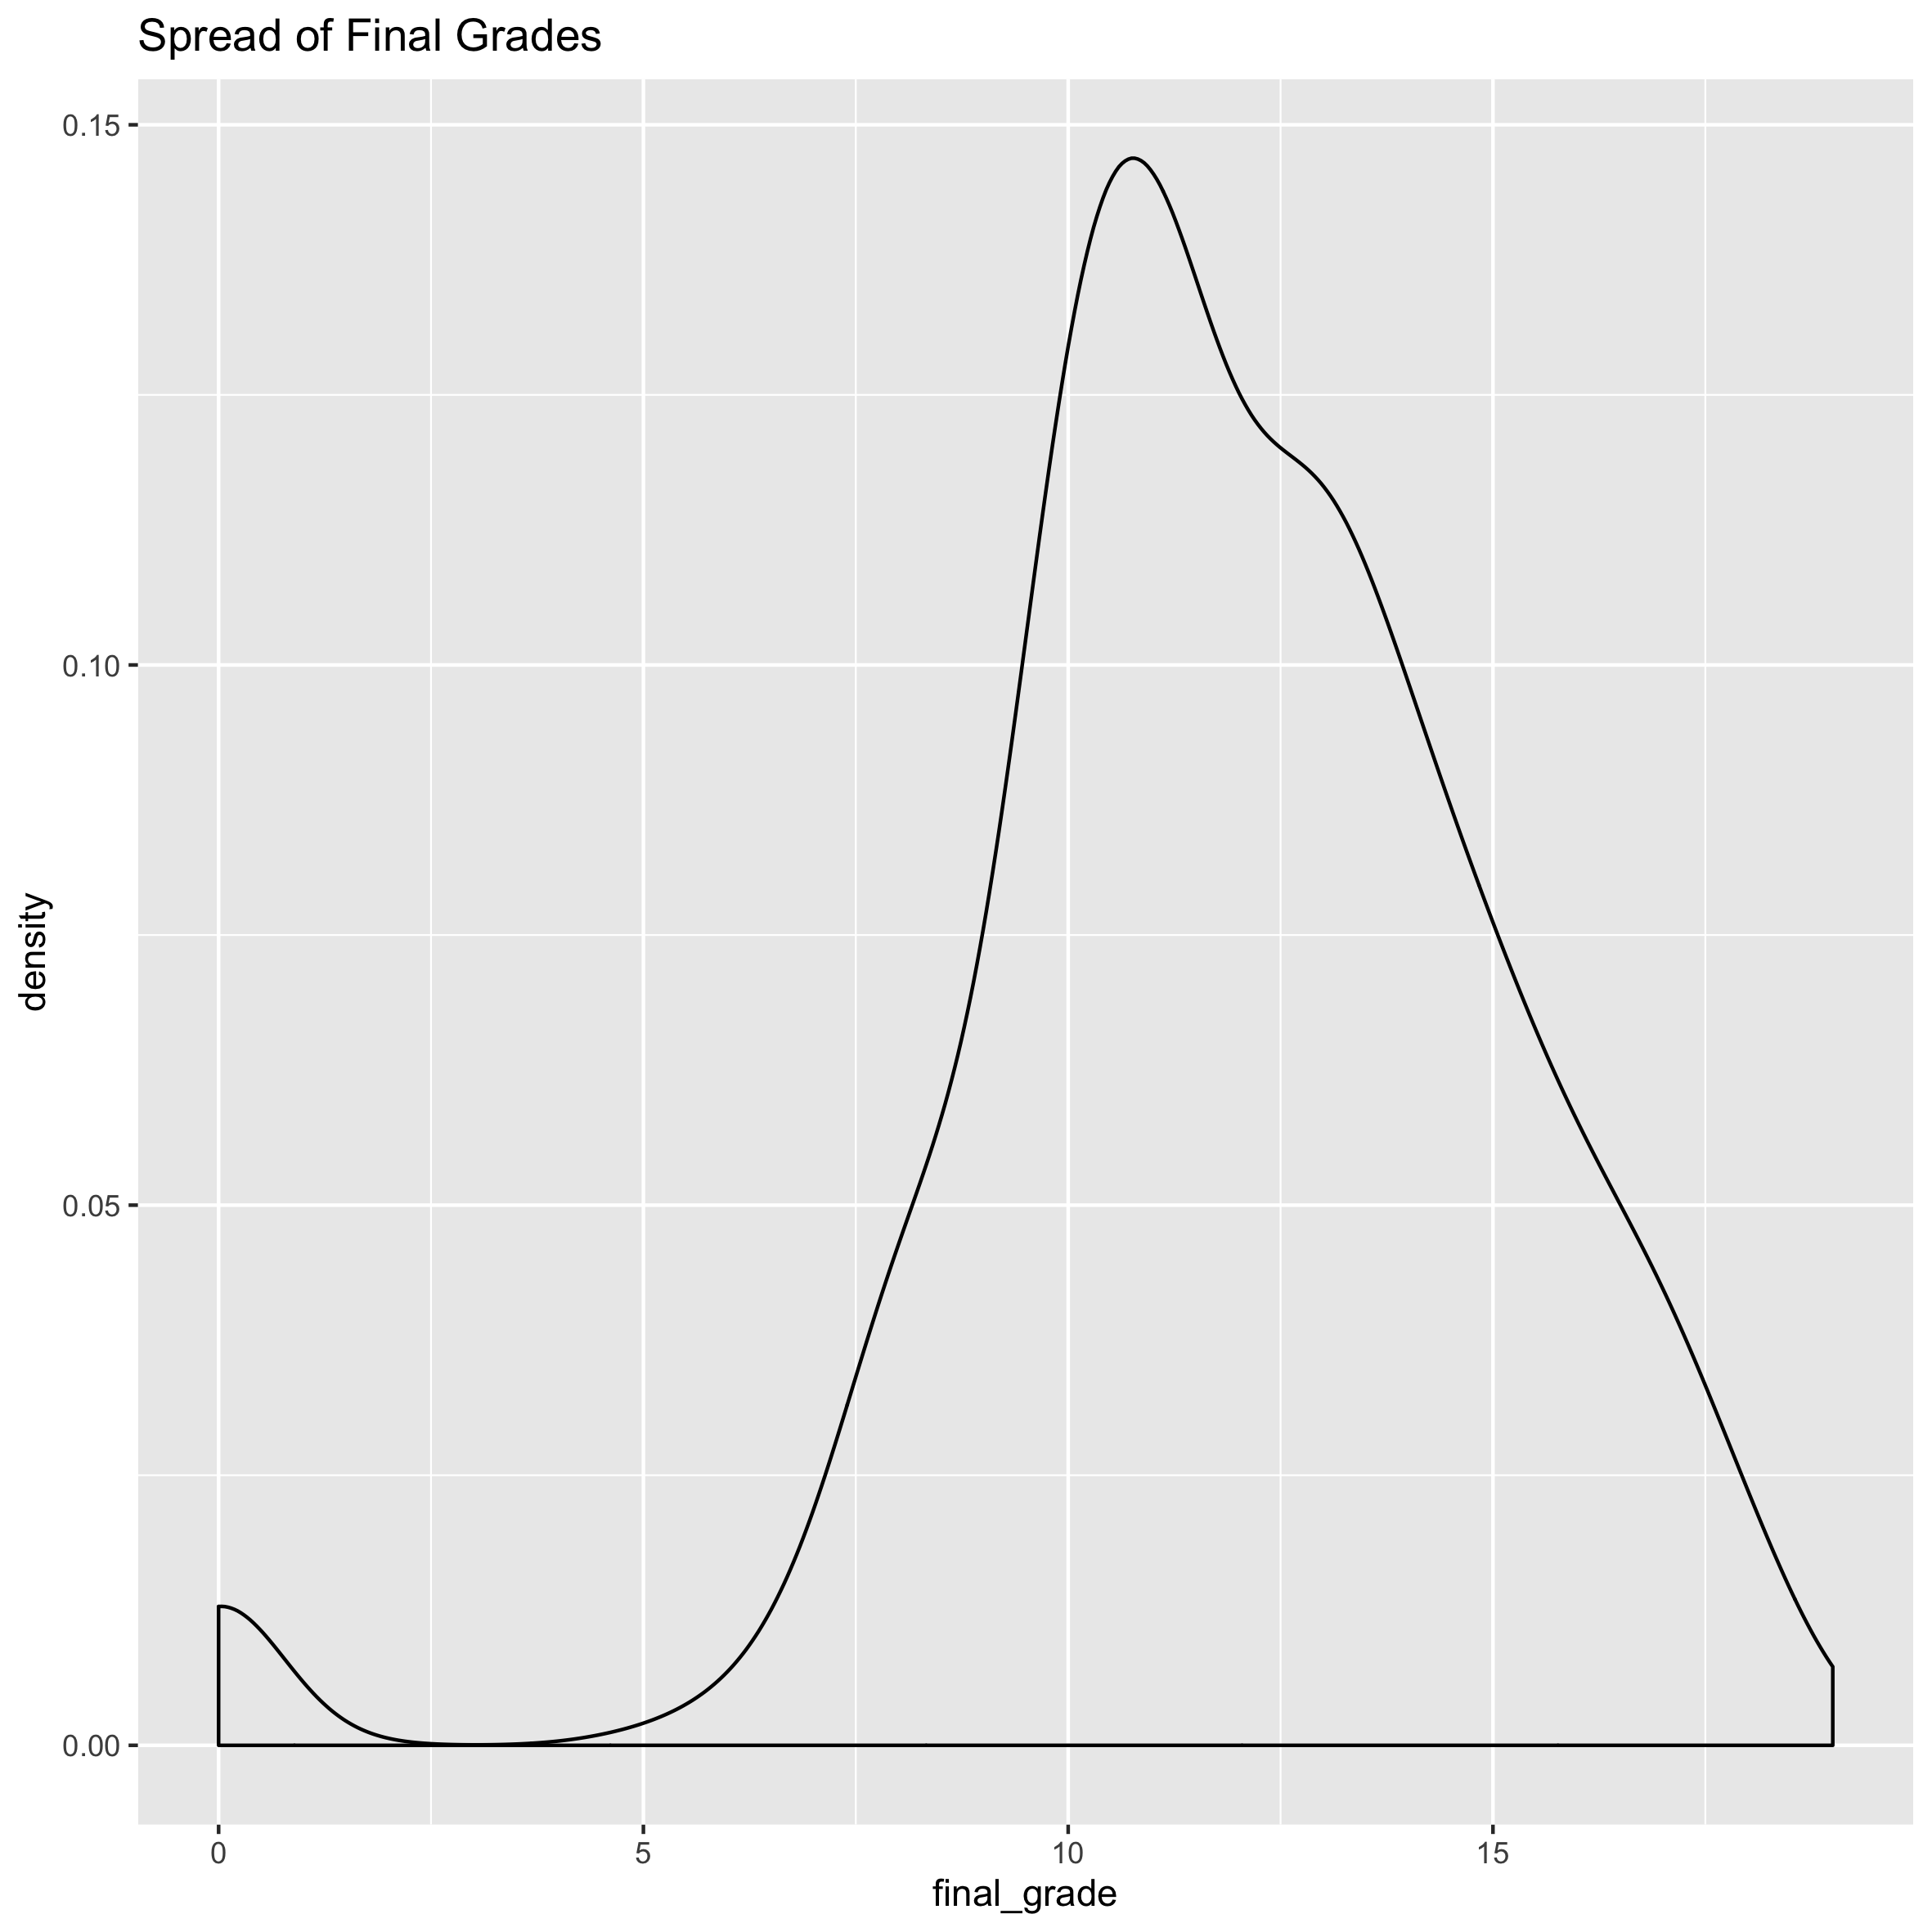
\includegraphics[width=0.8\textwidth,height=\textheight]{images/density_plot_grades.png}

The distribution of grades appear to be a bit left skewed.

\hypertarget{other-variables-that-may-affect-data}{%
\paragraph{Other variables that may affect
data}\label{other-variables-that-may-affect-data}}

Let's look at potential confounding factors like sex of the student,
parental status and family support and their spread in average final
grades

\#\#\#\#\#``Potential Confounding factors and grades''

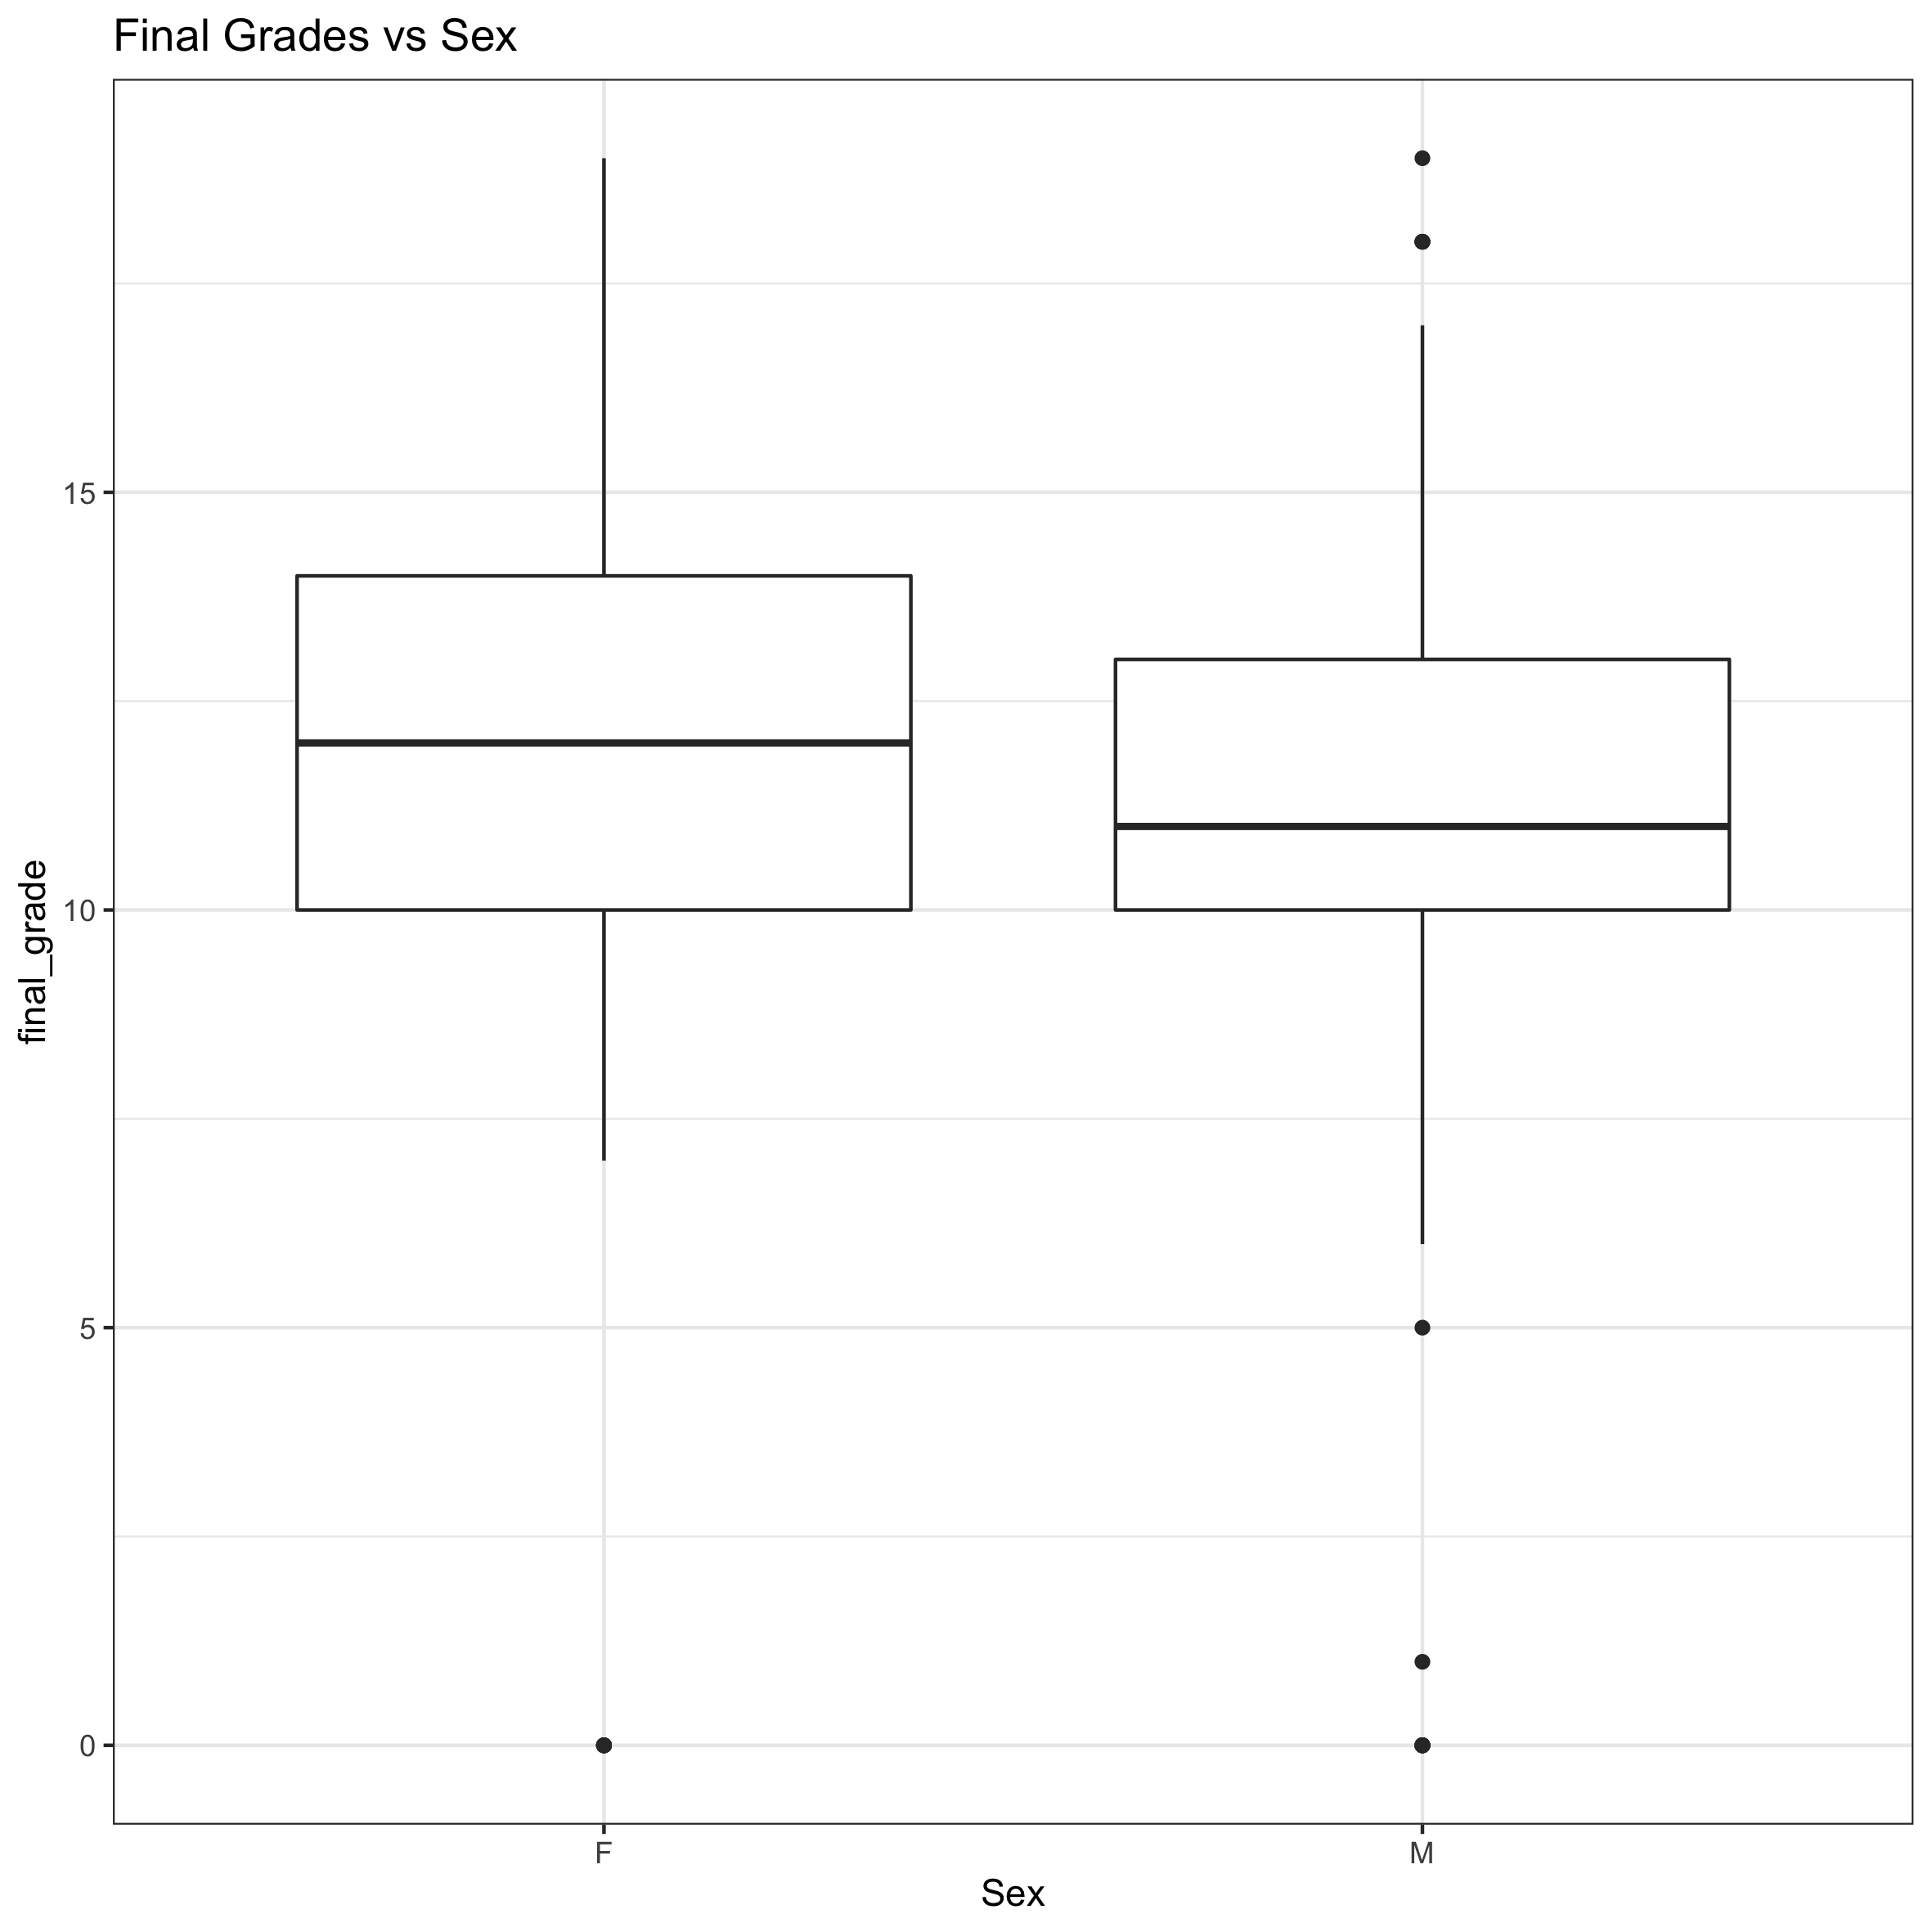
\includegraphics[width=0.8\textwidth,height=\textheight]{images/Final Grade vs Sex.png}~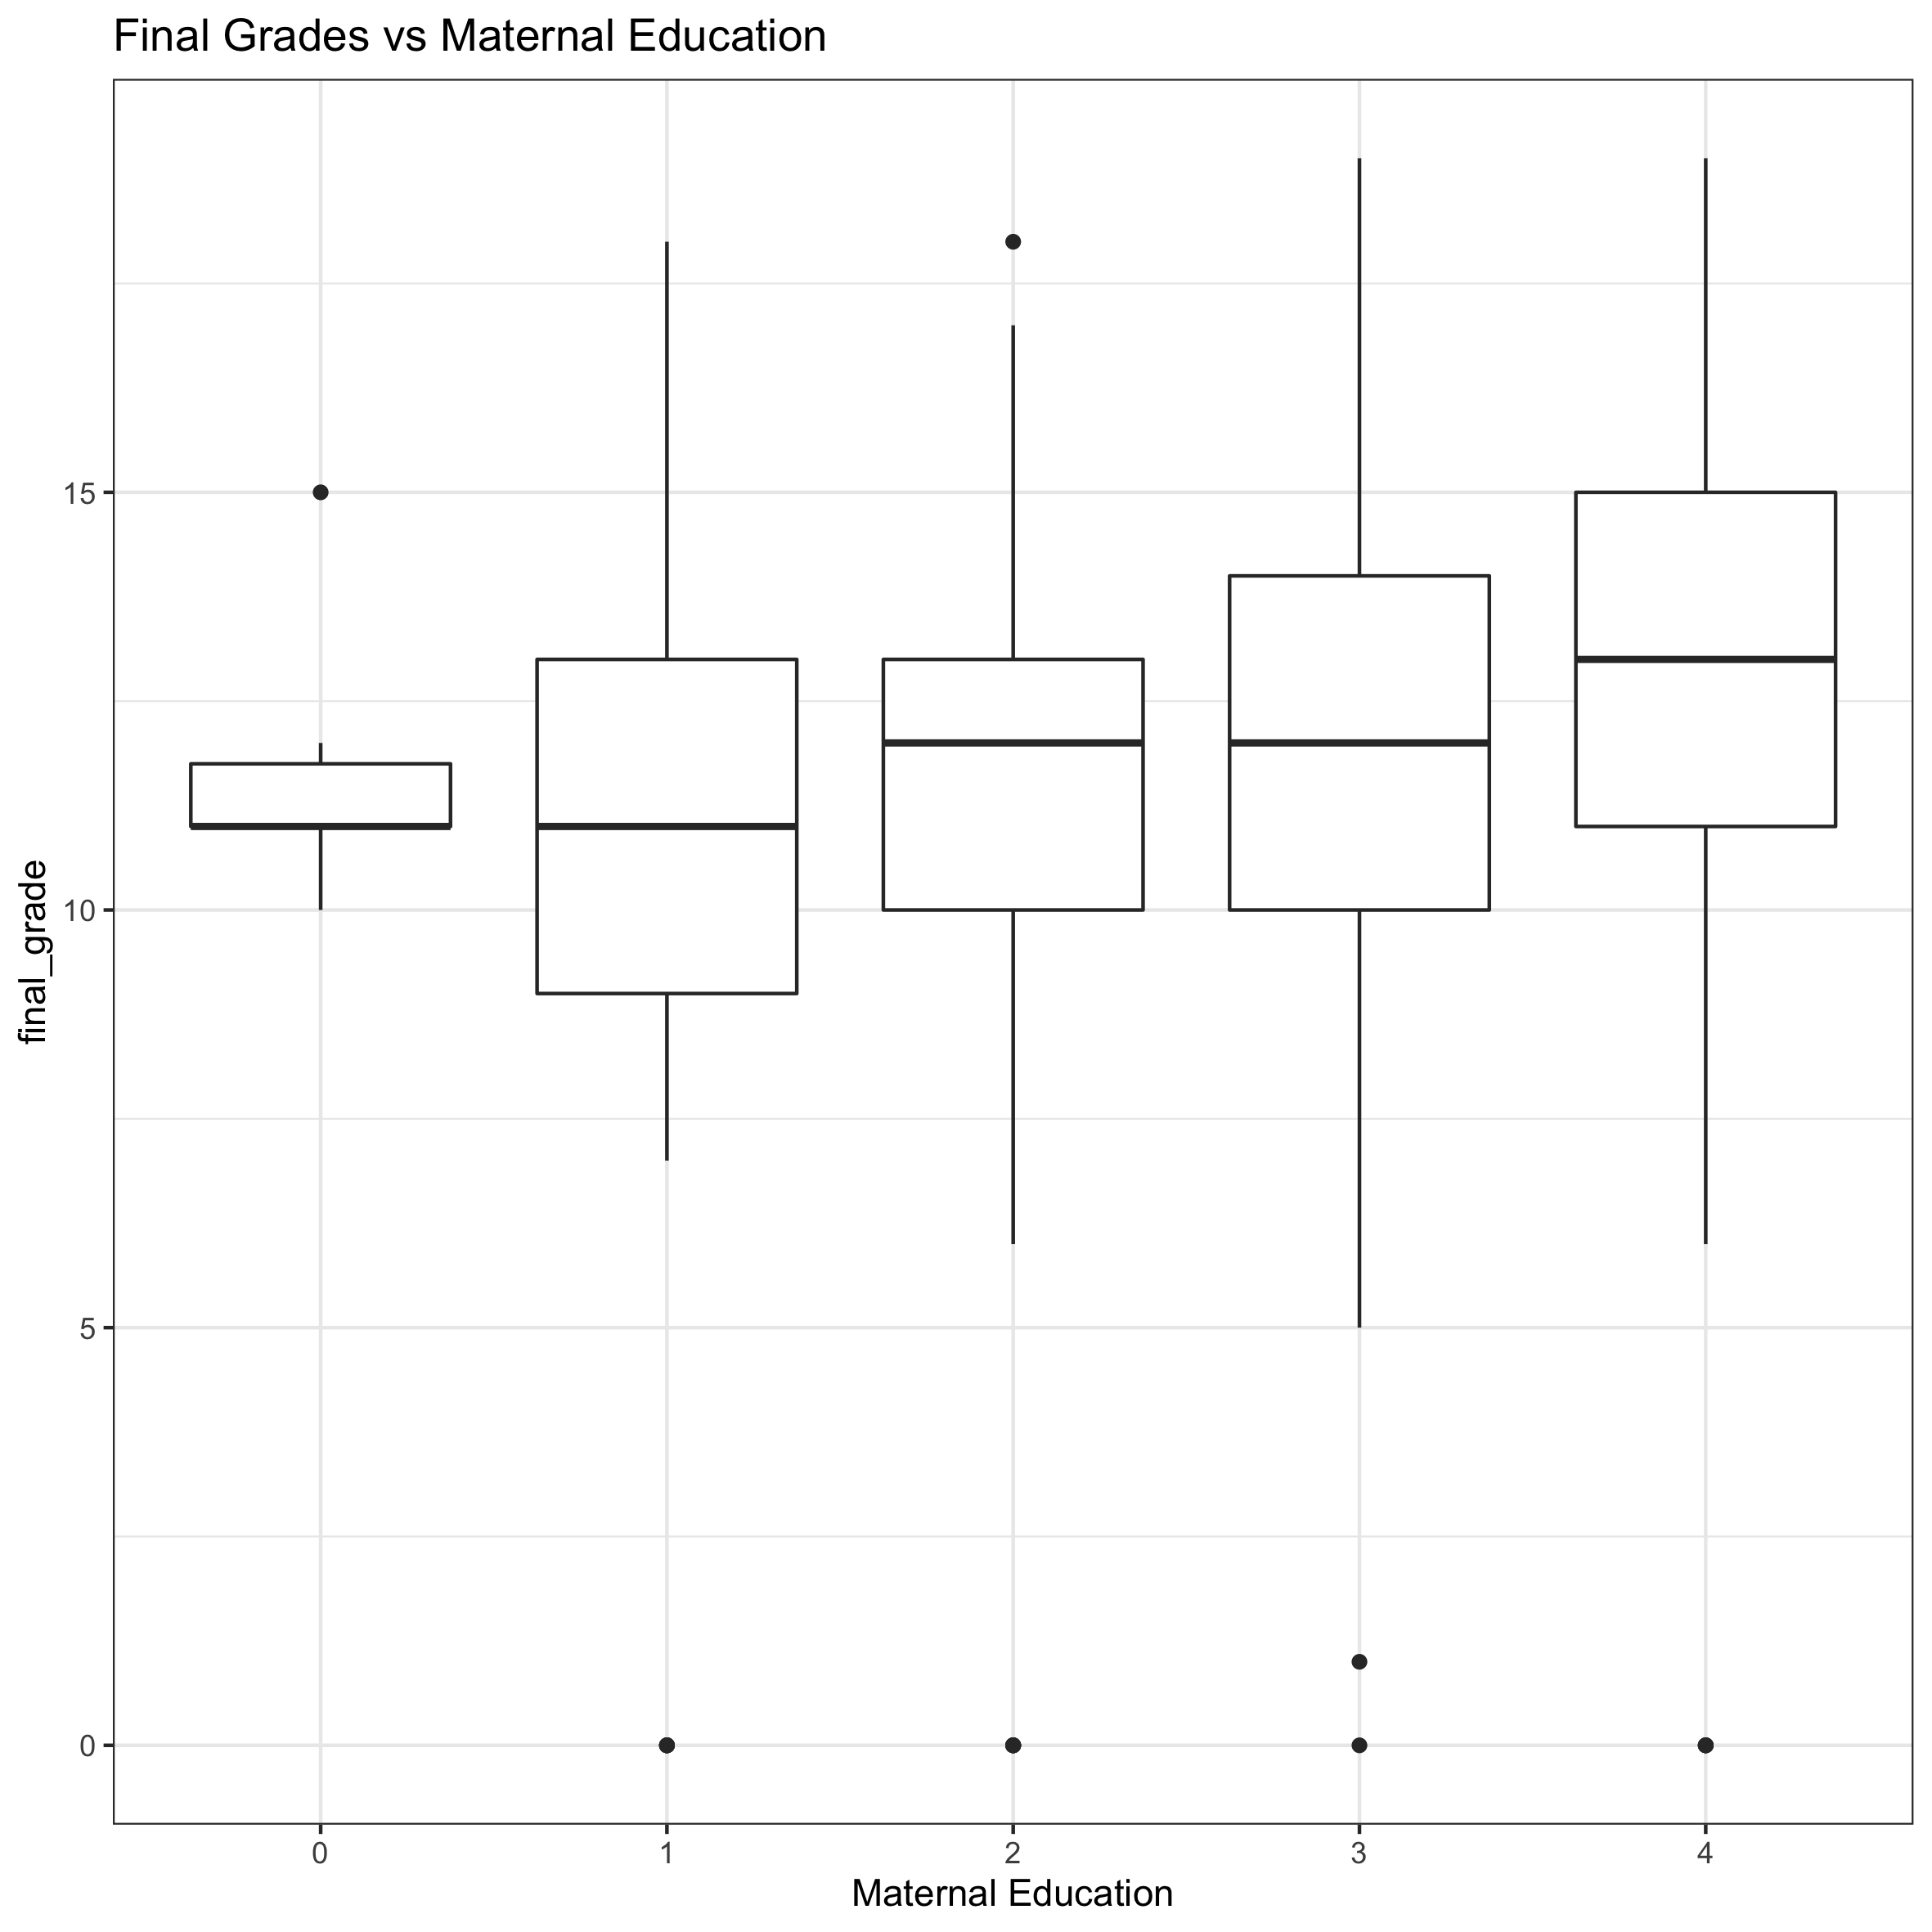
\includegraphics[width=0.8\textwidth,height=\textheight]{images/Final Grade vs Maternal Education.png}
\includegraphics[width=0.8\textwidth,height=\textheight]{images/Final Grade vs Parental status.png}~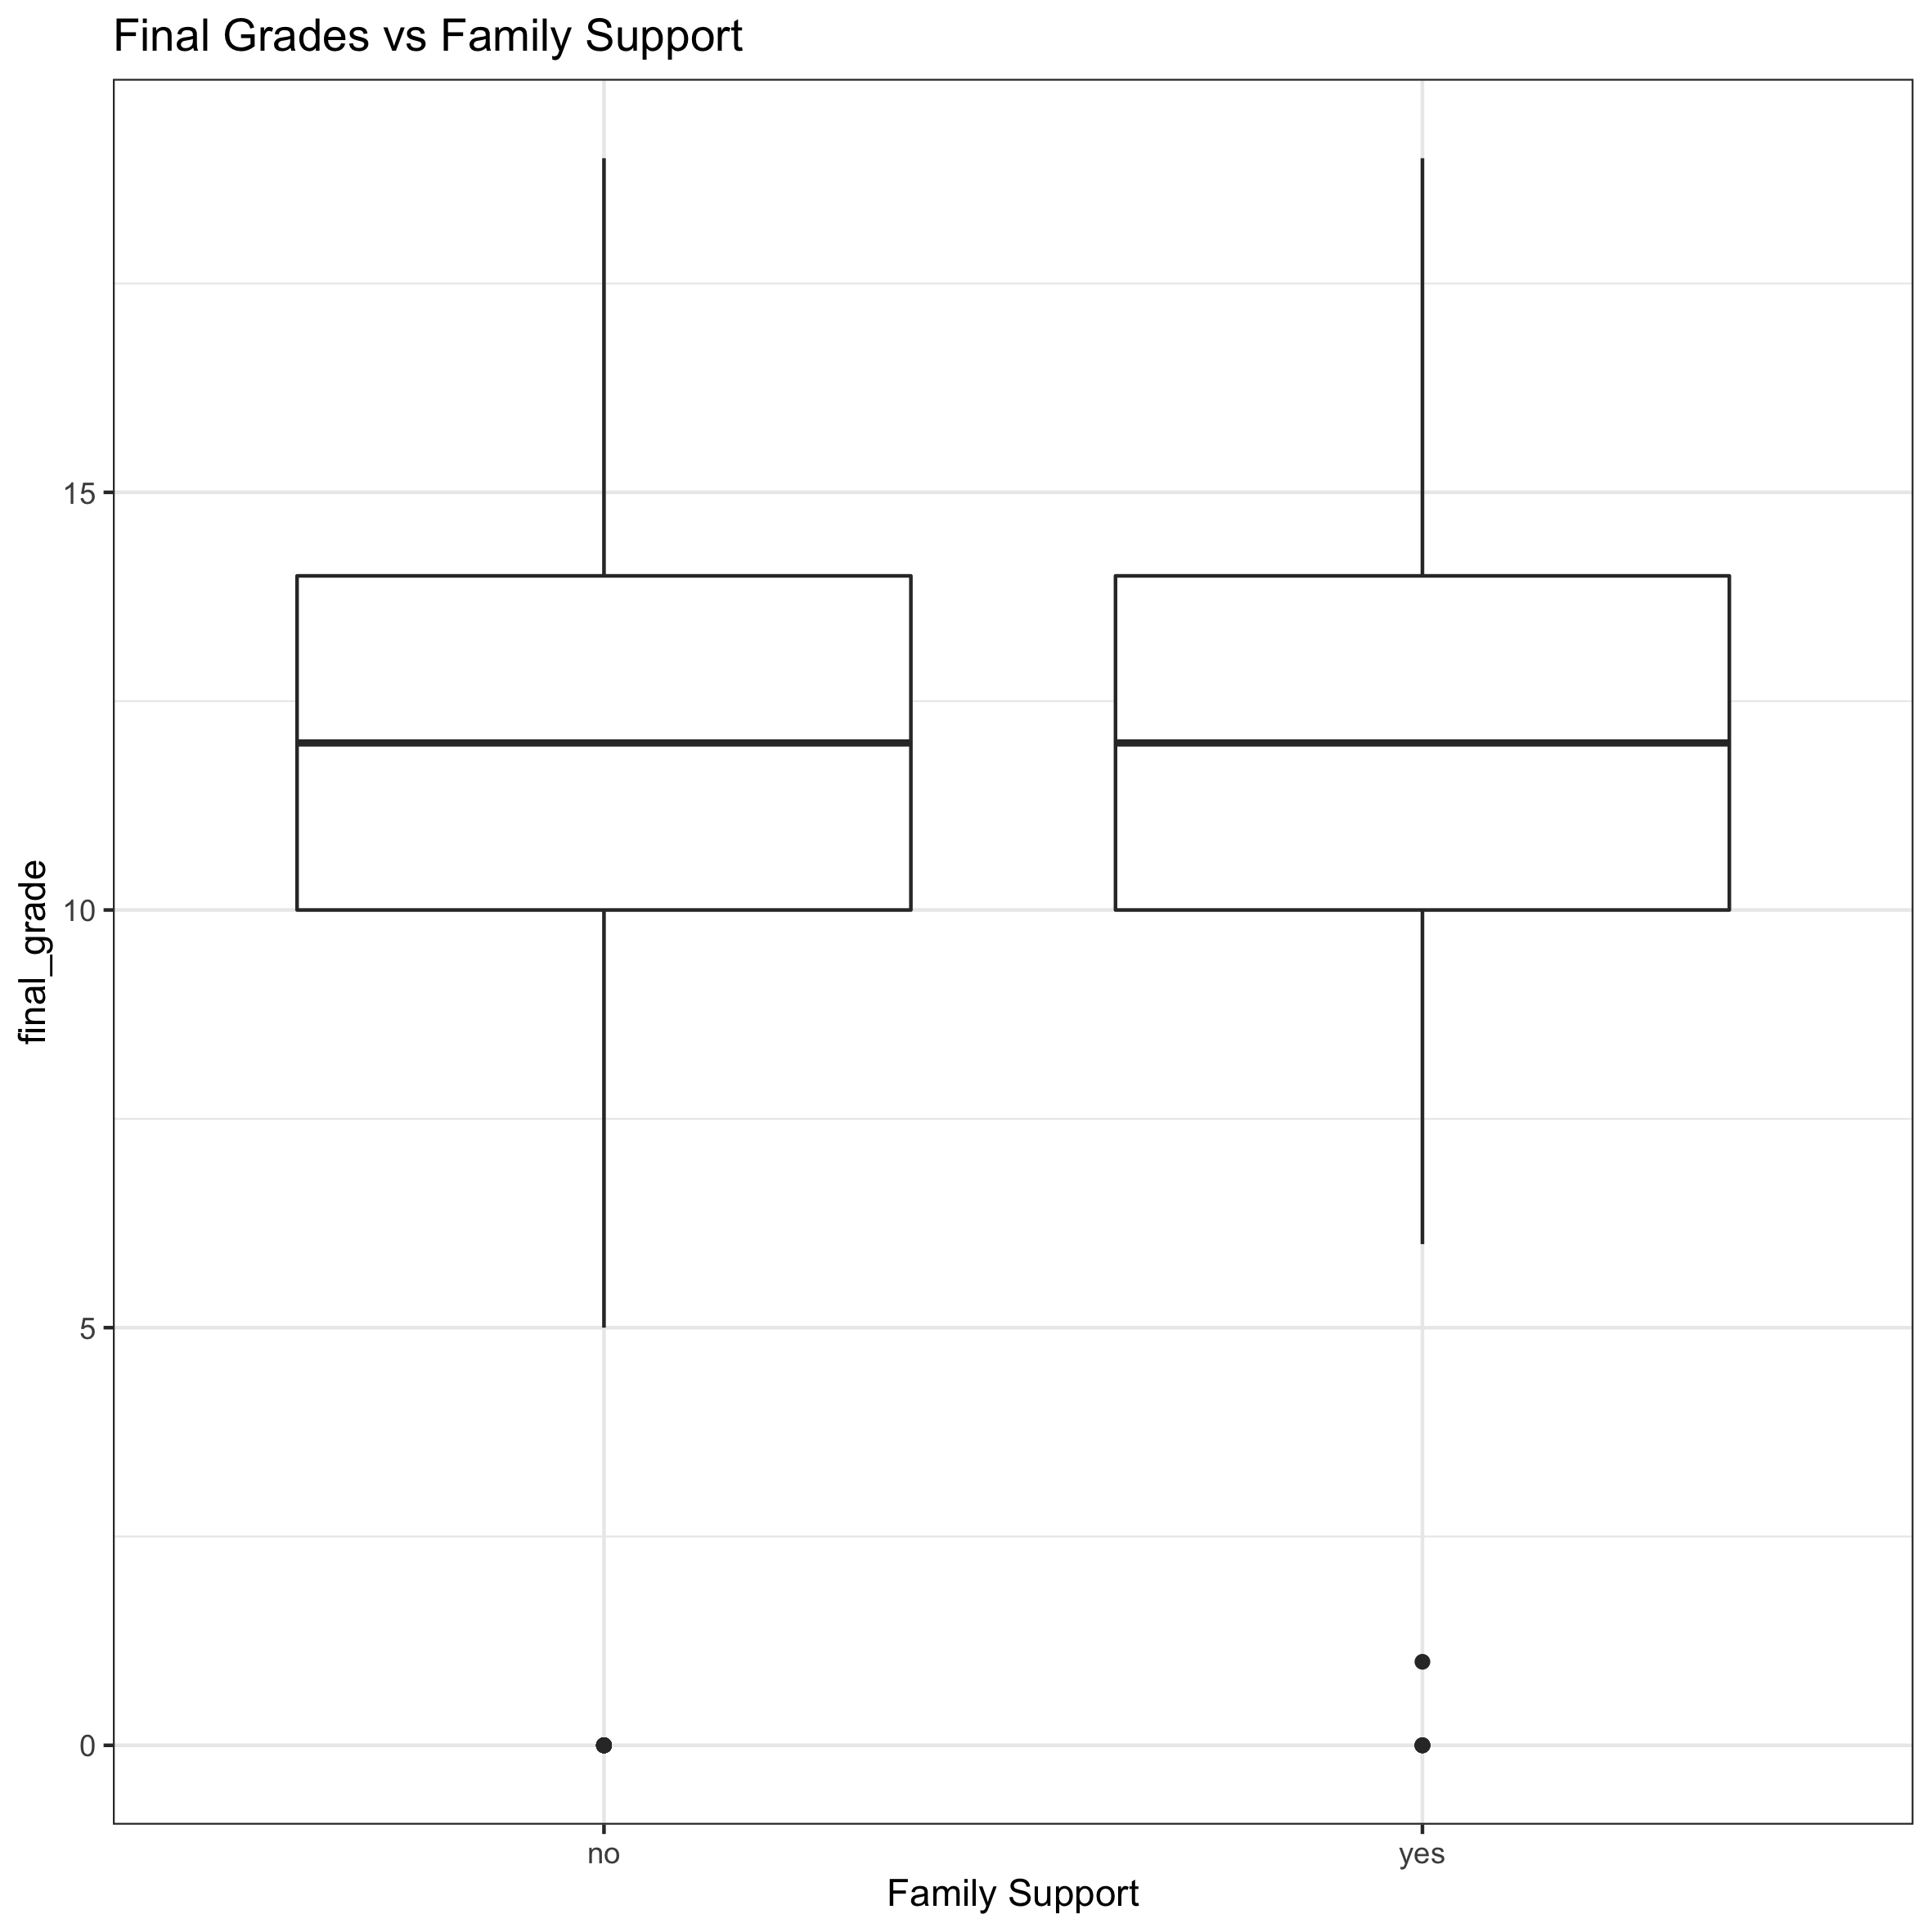
\includegraphics[width=0.8\textwidth,height=\textheight]{images/Final Grade vs Family Support.png}
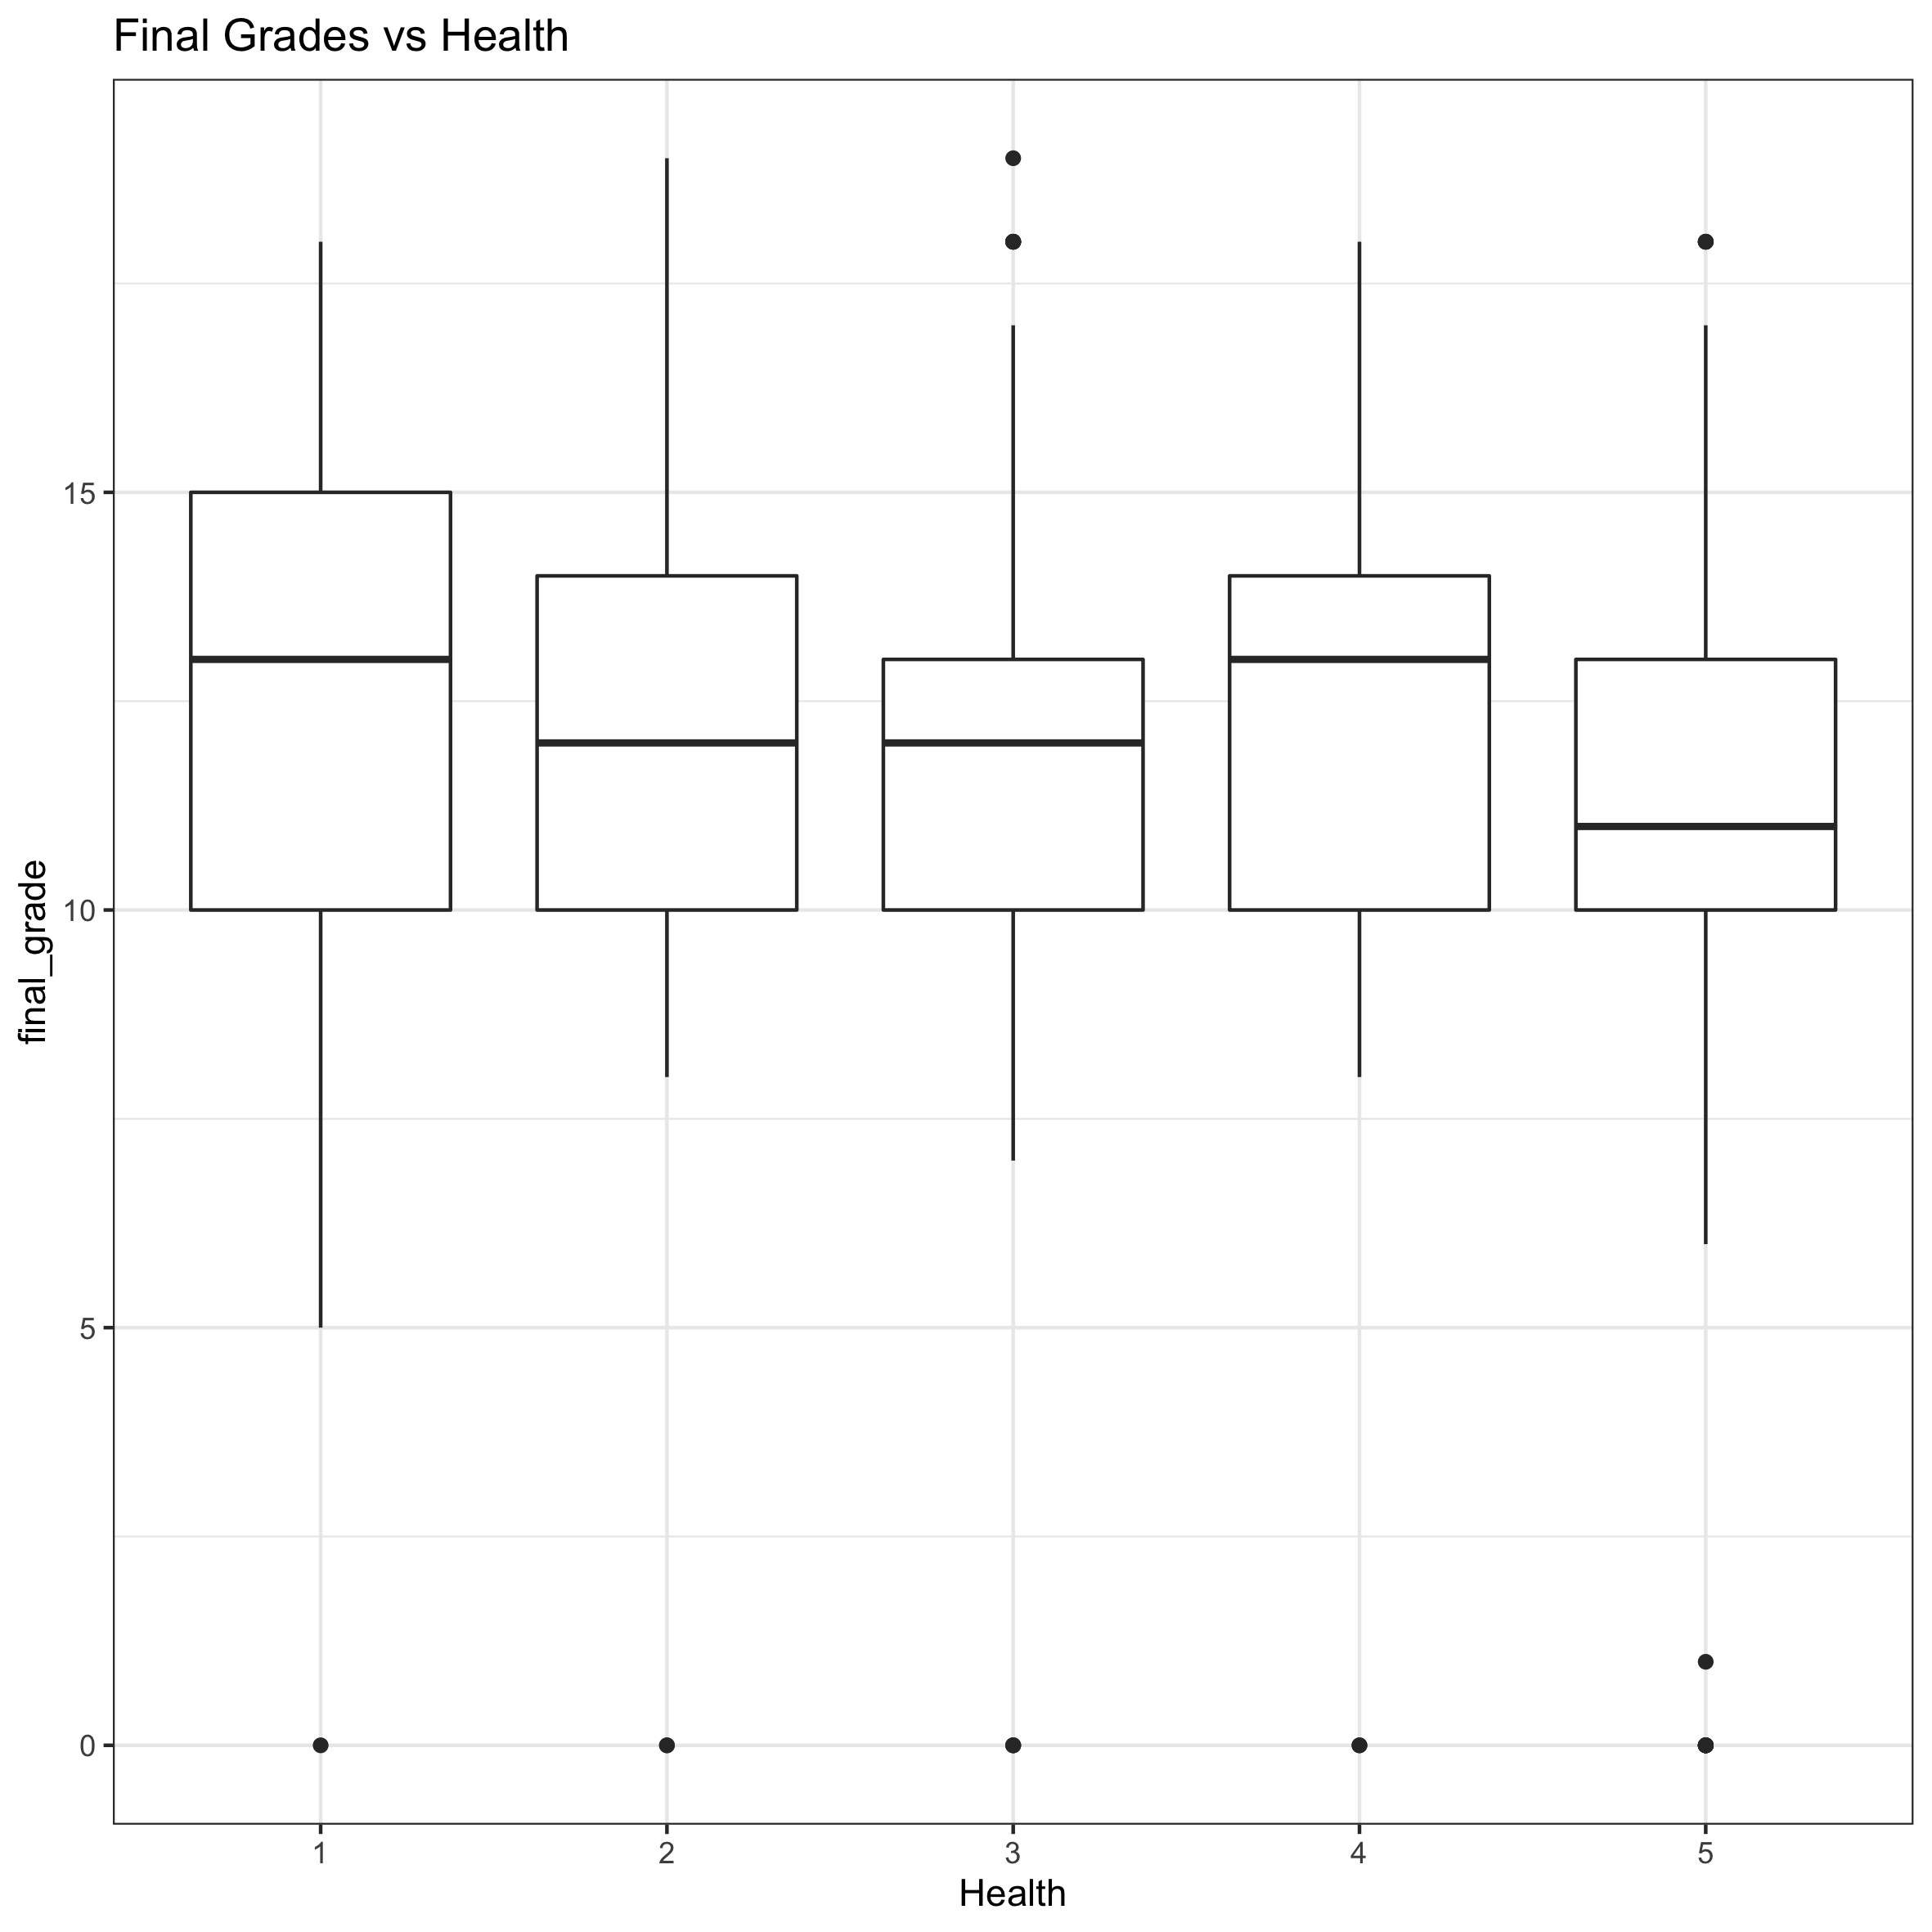
\includegraphics[width=0.8\textwidth,height=\textheight]{images/Final Grade vs Health.png}

It doesn't look like there is a huge difference between the grades in
males compared to females. Males have a slighly lower average, but
overall are similar. This is good because it will not be a huge confound
in the data.Also family support and parental status have similar average
values.

\hypertarget{research-question}{%
\subsection{Research Question:}\label{research-question}}

In this analysis, I will use linear regression to determine the
relationship between alcohol use, either weekend, weekday (workday) or
both and final grades (G3) for students. I chose the final grades as a
output variable because it is more resistant to short term effects
because it depends on work throughout the term.

\hypertarget{plan-of-action}{%
\subsection{Plan of Action:}\label{plan-of-action}}

I will remove those with very bad health status (1), as to reduce
confounds in the data. My main focus is on the alcohol use categories
and final grades, so I will probably ignore the other factors.I will
then perform linear regression analysis and plot a regression line using
the relevant variables.

\hypertarget{methods}{%
\subsection{Methods}\label{methods}}

I performed a multivariate simple linear regression using the lm
package, after removing the very bad health status(1). I used workday
alcohol and weekend alcohol as covariates and looked at interaction
between these 2 as well.

\begin{Shaded}
\begin{Highlighting}[]
\NormalTok{lm_model <-}\StringTok{ }\KeywordTok{readRDS}\NormalTok{(}\KeywordTok{here}\NormalTok{(}\StringTok{"data"}\NormalTok{,}\StringTok{"lm_model_alc.RDS"}\NormalTok{))}
\end{Highlighting}
\end{Shaded}

\hypertarget{results}{%
\subsection{Results}\label{results}}

Let's look at our linear model results.

\begin{Shaded}
\begin{Highlighting}[]
\KeywordTok{tidy}\NormalTok{(lm_model)}
\end{Highlighting}
\end{Shaded}

\begin{verbatim}
## # A tibble: 4 x 5
##   term                                    estimate std.error statistic  p.value
##   <chr>                                      <dbl>     <dbl>     <dbl>    <dbl>
## 1 (Intercept)                               13.7       0.619     22.2  1.21e-78
## 2 dataset$workday_alc                       -1.16      0.478     -2.44 1.52e- 2
## 3 dataset$weekend_alc                       -0.370     0.208     -1.78 7.61e- 2
## 4 dataset$workday_alc:dataset$weekend_alc    0.161     0.117      1.38 1.69e- 1
\end{verbatim}

\begin{Shaded}
\begin{Highlighting}[]
\KeywordTok{glance}\NormalTok{(lm_model)}
\end{Highlighting}
\end{Shaded}

\begin{verbatim}
## # A tibble: 1 x 11
##   r.squared adj.r.squared sigma statistic p.value    df logLik   AIC   BIC
##       <dbl>         <dbl> <dbl>     <dbl>   <dbl> <int>  <dbl> <dbl> <dbl>
## 1    0.0437        0.0385  3.16      8.45 1.70e-5     4 -1434. 2877. 2899.
## # ... with 2 more variables: deviance <dbl>, df.residual <int>
\end{verbatim}

The only result that seems to be significant is the workday alcohol with
grades. The interaction term is not significant, thus we can point that
workday alcohol affects grades as a main effect. There appprea

\hypertarget{residual-plots}{%
\subsubsection{Residual Plots:}\label{residual-plots}}

Let's look at qqplots of the residulat and residual vs fitted plots.

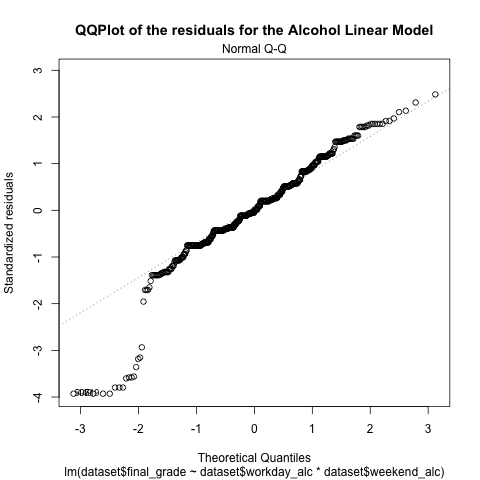
\includegraphics[width=0.8\textwidth,height=\textheight]{images/residual_plot_qq.png}~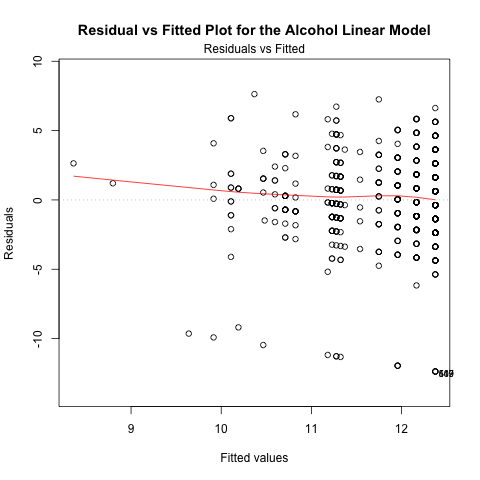
\includegraphics[width=0.8\textwidth,height=\textheight]{images/residual_fitted_plot.png}

The residuals do not all fall onto the qqplot and thus are not fully
normally distributed.

\hypertarget{discussionconclusions}{%
\subsection{Discussion/Conclusions}\label{discussionconclusions}}

The only predictor variable that was significant was workday alcohol
which had a negative association with final grades. This is in line with
Balsa et al.'s study, which saw a significant, but small negative
association with alcohol and grades, specifically for males. In my case,
I did not separate by gender, which could be a future analysis. Also, I
think including other covariates like family support in the future would
be a good idea. Finally, given the qqplot, it would be best to
potentially change the model from a simple linear regression that treats
the predictor of alcohol use as a numeric, into a more complex model
that treats this predictor as a categorical and uses dummy variables.

\end{document}
